\chapter{研究の準備}\label{cha:Preparation}

本章では、本研究におけるシステム仕様書と章立ての位置づけ、および本研究で提案するシステム仕様書章立て生成プロンプトの基礎となる技術的要素について述べる。


\section{システム仕様書}
\label{sec:system_spec}

\subsection{本研究におけるシステム仕様書の位置づけ}
\label{subsec:system_spec_position}

本研究でモデルケースとするシステム開発の流れを、図\ref{fig:system_development_process}に示す\cite{vmodel}。

\begin{figure}[tp]
  \centering
  % \fbox{
  \includegraphics[width=0.95\textwidth]{images/vmodel.pdf}
  % }
  \captionof{figure}{本研究でモデルケースとするシステム開発の流れ}
  \label{fig:system_development_process}
\end{figure}

本研究におけるシステム仕様書は、顧客の要求や口頭での指示といった曖昧な情報を、初めて具体的な要件および設計情報として文書化する役割を担い、システム開発における最初の成果物として位置付けている。


\subsection{本研究におけるシステム仕様書作成の目的}
\label{subsec:system_spec_purpose}

システム仕様書は、以下の2つの目的を達成するための成果物と定義する。
\begin{itemize}
  \item \textbf{実装者への指針}:
  システム開発の経験の少ない実装者であっても、システム仕様書を読むことでシステムの挙動を正しく理解し、実装に着手できること。
  \item \textbf{テスト担当者への指針}:
  システムの内部構造(ソースコード)を知らないテスト担当者が、システム仕様書に記載された正常系、および異常系のエラー条件に従って、ブラックボックステストの項目を作成できること。
\end{itemize}


\subsection{本研究におけるシステム仕様書の記述内容}
\label{subsec:system_spec_content}

本研究におけるシステム仕様書の記述内容としては、画面レイアウトや操作フローといった外部仕様\cite{rasinban}を記し、内部仕様\cite{rasinban}は含まない。

\subsection{システム仕様書の章立て}
\label{subsec:general_spec}

本研究では、章立ては以下の6つの要素からなる。
\begin{itemize}
    \item 章番号(1. 2. 3. ...)
    \item 章タイトル
    \item 節番号(1.1. 1.2. ...)
    \item 節タイトル
    \item 項番号(1.1.1. 1.1.2. ...)
    \item 項タイトル
\end{itemize}

図\ref{fig:outline_example}に、システム仕様書の章立ての例を示す。
これは、BMP画像を指定された数に分割し保存するアプリケーションである、BMP画像分割アプリのシステム仕様書の章立てである。

\begin{figure}[tp]
  \centering
  \fbox{
    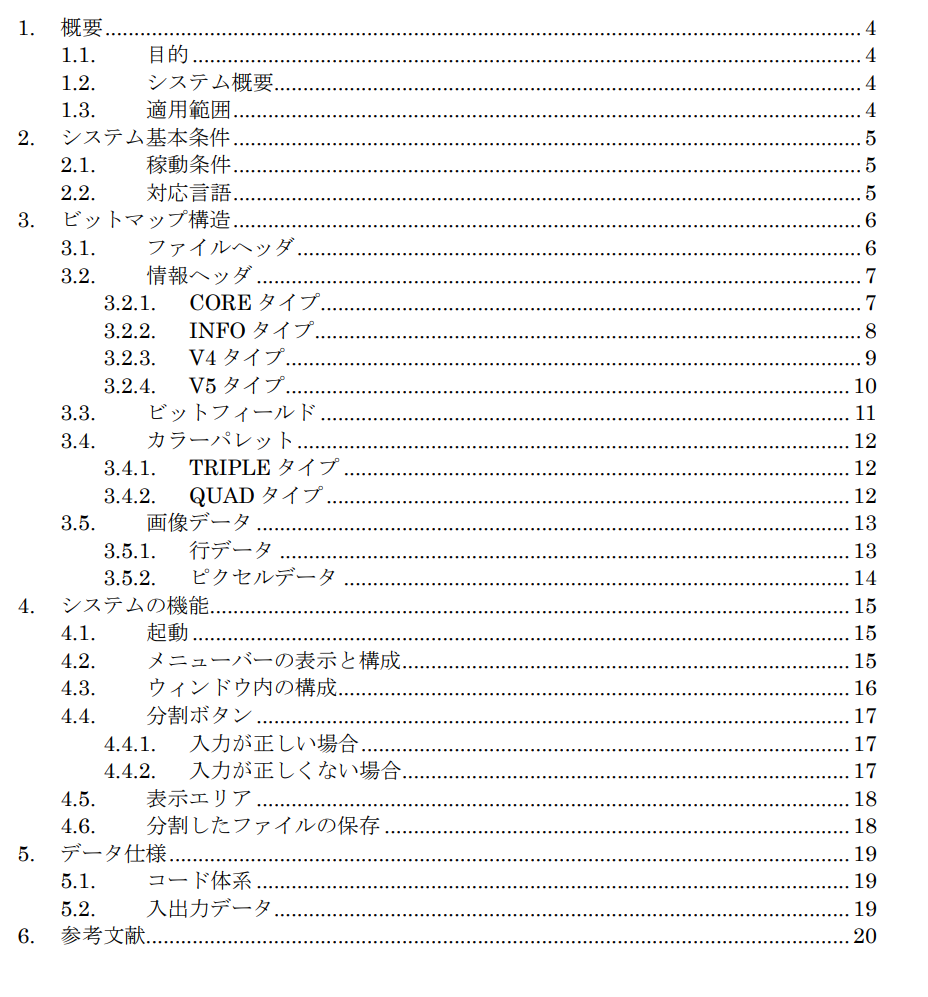
\includegraphics[width=0.95\textwidth]{images/システム仕様書章立ての例.png}
  }
  \captionof{figure}{BMP画像分割アプリのシステム仕様書の章立ての例}
  \label{fig:outline_example}
\end{figure}

\subsection{一般的な章立ての構成要素}
\label{subsec:general_outline}

システム仕様書の章立ては、対象とするシステムの特性や組織の標準により異なるが、システム仕様書として作成される文書には、システムが提供する機能や振る舞いを網羅的に記述することが求められる。
国際的な標準としては、IEEE830 (Recommended Practice for Software Requirements Specifications)\cite{ieee830} が広く知られており、機能要件、外部インターフェース、パフォーマンスなどの非機能要件を記述することが推奨されている。

図\ref{fig:ieee830}に、IEEE830に基づくシステム仕様書の章立てに含むべき項目を示す。

% \begin{enumerate}
%     \item \textbf{システム概要}
%     \begin{itemize}
%         \item システムの目的
%         \item 背景
%         \item 全体像
%     \end{itemize}
%     \item \textbf{機能要件}
%     \begin{itemize}
%         \item システムが提供する機能の一覧
%         \item 各機能の詳細な振る舞い(入力・処理・出力)
%     \end{itemize}
%     \item \textbf{ユーザーインターフェース (UI)}
%     \begin{itemize}
%         \item 画面レイアウト
%         \item 画面遷移図
%         \item 操作フロー
%     \end{itemize}
%     \item \textbf{データ要件}
%     \begin{itemize}
%         \item 扱うデータの定義(ER図やデータディクショナリ)
%     \end{itemize}
%     \item \textbf{外部インターフェース}
%     \begin{itemize}
%         \item 外部システムとの連携仕様
%         \item API定義
%     \end{itemize}
%     \item \textbf{非機能要件}
%     \begin{itemize}
%         \item セキュリティ
%         \item 性能
%         \item 信頼性
%         \item 制約事項
%     \end{itemize}
% \end{enumerate}


\begin{figure}[tp]
\begin{tcolorbox}[
  colback=white,
  colframe=black,
  fonttitle=\bfseries,
]
\footnotesize
\ttfamily
\fontsize{10}{11}\selectfont
\begin{verbatim}
1. はじめに
   1.1 本書の目的
   1.2 対象範囲
   1.3 用語定義・略語
   1.4 参考資料
   1.5 本書の構成

2. システム概要
   2.1 システムの全体像
    2.1.1 システム間インターフェース
    2.1.2 画面インターフェース
    2.1.3 ハードウェア構成
    2.1.4 ソフトウェア構成
    2.1.5 ネットワーク構成
    2.1.6 リソース制約
    2.1.7 運用環境
    2.1.8 設置条件
   2.2 システムの主な機能
   2.3 想定利用者
   2.4 制約事項
   2.5 前提条件および依存関係
   2.6 将来対応事項

3. 詳細要件
   3.1 外部インターフェース仕様
   3.2 機能要件
   3.3 性能要件
   3.4 データベース要件
   3.5 設計上の制約事項
   3.6 システム品質特性
    3.6.1 信頼性
    3.6.2 可用性
    3.6.3 セキュリティ
    3.6.4 保守性
    3.6.5 移植性
   3.7 その他の要件

4. 参考資料
   4.1 索引
   4.2 付録
\end{verbatim}
\end{tcolorbox}
\par\vspace{-20pt}
\captionof{figure}{IEEE830に基づくシステム仕様書の章立てに含むべき項目}
\label{fig:ieee830}
\end{figure}


% \begin{enumerate}
%     \item \textbf{はじめに}
%     \begin{enumerate}[label=1.\arabic*]
%         \item 本書の目的
%         \item 対象範囲
%         \item 用語定義・略語
%         % \item 参考資料
%         \item 本書の構成
%     \end{enumerate}

%     \item \textbf{システム概要}
%     \begin{enumerate}[label=2.\arabic*]
%         \item システムの全体像
%         \begin{enumerate}[label=2.1.\arabic*]
%             \item システム間インターフェース
%             \item 画面インターフェース
%             \item ハードウェア構成
%             \item ソフトウェア構成
%             \item ネットワーク構成
%             \item リソース制約
%             \item 運用環境
%             \item 設置条件
%         \end{enumerate}
%         \item システムの主な機能
%         \item 想定利用者
%         \item 制約事項
%         \item 前提条件および依存関係
%         \item 将来対応事項
%     \end{enumerate}

%     \item \textbf{詳細要件}
%     \begin{enumerate}[label=3.\arabic*]
%         \item 外部インターフェース仕様
%         \item 機能要件
%         \item 性能要件
%         \item データベース要件
%         \item 設計上の制約事項
%         \item システム品質特性
%         \begin{enumerate}[label=3.6.\arabic*]
%             \item 信頼性
%             \item 可用性
%             \item セキュリティ
%             \item 保守性
%             \item 移植性
%         \end{enumerate}
%         \item その他の要件
%     \end{enumerate}

%     \item \textbf{参考資料}
%     \begin{enumerate}[label=4.\arabic*]
%         \item 索引
%         \item 付録
%     \end{enumerate}
% \end{enumerate}


本研究で対象とするシステム仕様書の章立ては、標準的な構成要素を踏まえつつ、対象システム特有の要件を反映した、章、節、項も含めた構成を目指す。


\section{Large Language Models (LLM)}
\label{sec:llm}

Large Language Models (大規模言語モデル)\cite{whatllm}は、膨大なテキストデータと高度なディープラーニング技術を用いて構築された、自然言語処理分野における技術である。

本研究では、OpenAI\cite{openai}社が提供するLLMであるGPT-5.2\cite{gpt52}を搭載したChatGPT\cite{chatgpt}を、システム仕様書章立ての生成に用いる。

\section{プロンプトエンジニアリング}
\label{sec:prompt_engineering}

プロンプトエンジニアリングとは、LLMにタスクの実行を命令する際、LLMから望ましい出力を得るために、入力するプロンプトを設計、および最適化する技術のことである\cite{prompt_engineering}。
LLMの性能を最大限に引き出すためには、モデルの特性を理解して、適切なプロンプトを構築し、入力する必要がある。以降、本研究で用いるプロンプトエンジニアリングに関連する主要な手法について述べる。

\subsection{Few-shot Prompting}
\label{subsec:few_shot}

Few-shot Prompting\cite{fewshot}は、いくつかの入力例と出力例のペアを提示することで、LLMにタスクの意図を理解させて、望ましい形式や内容で出力を生成できるよう誘導する手法である。
図\ref{fig:few}に、Few-shot Promptingの具体例を示す。

図\ref{fig:few}のプロンプト例における、入力例は、「フランスの首都」、「日本の首都」、「アメリカの首都」、「イギリスの首都」であり、出力例は、「パリ」、「東京」、「ワシントンD.C」、「ロンドン」である。

\begin{figure}[tp]
\begin{tcolorbox}[
  colback=white,
  colframe=blue,
  fonttitle=\bfseries,
]
\footnotesize
\ttfamily
\fontsize{10}{11}\selectfont
\begin{verbatim}
フランスの首都：パリ
日本の首都：東京
アメリカの首都：ワシントンD.C.
イギリスの首都：ロンドン
では、ブラジルの首都は？
\end{verbatim}
\end{tcolorbox}
% \par\vspace{-20pt}
\captionof{figure}{Few-shot Promptingの例}
\label{fig:few}
\end{figure}

% \begin{table}[tp]
%   \caption{図\ref{fig:few}における入力例と出力例}
%   \label{tb:inoutexample}
%   \centering
%   \begin{tabular}{|c|c|}
%     \hline
%     \textbf{入力例} & \textbf{出力例} \\
%     \hline\hline
%     フランスの首都 & パリ \\
%     \hline
%     日本の首都 & 東京 \\
%     \hline
%     アメリカの首都 & ワシントンD.C. \\
%     \hline
%     イギリスの首都 & ロンドン \\
%     \hline
%   \end{tabular}
% \end{table}


\subsection{One-shot Prompting}
\label{subsec:one_shot}

One-shot Prompting\cite{oneshot}は、1つの入力例と出力例のペアを提示することで、LLMにタスクの意図を理解させて、望ましい形式や内容で出力を生成できるよう誘導する手法である。
図\ref{fig:one}に、One-shot Promptingの具体例を示す。この例では、「日本の首都」が入力例、「東京」が出力例となる。

\begin{figure}[tp]
\begin{tcolorbox}[
  colback=white,
  colframe=blue,
  fonttitle=\bfseries,
]
\footnotesize
\ttfamily
\fontsize{10}{11}\selectfont
\begin{verbatim}
日本の首都：東京。
では、ブラジルの首都は？
\end{verbatim}
\end{tcolorbox}
\captionof{figure}{One-shot Promptingの例}
\label{fig:one}
\end{figure}

\subsection{Zero-shot Prompting}
\label{subsec:zero_shot}

Zero-shot Prompting\cite{zeroshot}は、LLMに対してタスクの具体的な回答例を与えずに、指示のみでタスクを実行させる手法である。
図\ref{fig:zero}に、Zero-shot Promptingの具体例を示す。


\begin{figure}[tp]
\begin{tcolorbox}[
  colback=white,
  colframe=blue,
  fonttitle=\bfseries,
]
\footnotesize
\ttfamily
\fontsize{10}{11}\selectfont
\begin{verbatim}
ブラジルの首都は？
\end{verbatim}
\end{tcolorbox}
% \par\vspace{-20pt}
% \captionof{figure}{プロンプトの"役割付与"部分}
\captionof{figure}{Zero-shot Promptingの例}
\label{fig:zero}
\end{figure}



Tom Brownらの研究によると、Few-shot PromptingとOne-shot Promptingは、Zero-shot Promptingと比較して、出力の精度が高いとされる\cite{zeroonefew}。一方で、入力例と出力例のペアの作成が困難な場合は、Zero-shot Promptingが用いられる。

本研究でLLMの生成の対象としている章立ては、正解がなく、入力例と出力例を作成することが困難である。
そのため、本研究で提案するシステム仕様書章立て生成プロンプトは、Zero-shot Promptingの手法をベースとする。
ただし、LLMが生成する章立てが意図する章立ての構造とかけ離れたものにならないように、出力例として実際の開発現場で用いられている章立てのテンプレートをLLMに与える(詳細は第\ref{cha:Proposal}章で後述)。
したがって、本研究で提案するシステム仕様書章立て生成プロンプトは、具体的な入力例は与えないが、出力例は与えるため、One-shot Promptingを部分的に取り入れたプロンプトになっていると言える。

\section{プロンプトパターン}
\label{sec:prompt_patterns}

プロンプトパターンとは、特定の状況で課題解決に有効なプロンプトのパターンのことである\cite{nishino}。

本研究で提案するシステム仕様書章立て生成プロンプトでは、Jules Whiteらが提案するプロンプトパターンカタログ\cite{prompt-patterns}を参考に、以下の3つパターンを適用する。

\subsection{Persona Pattern}
\label{subsec:persona_pattern}

Persona Pattern (ペルソナパターン)は、LLMに対して特定の役割(ペルソナ)を与えることで、その役割に適した振る舞いや回答を促すパターンである\cite{prompt-patterns}。
Aobo Kongらの研究により、LLMに適切な役割を与えることで、回答の精度が向上することが示されている\cite{role_assignment}。

本研究で提案するシステム仕様書章立て生成プロンプトでは、文頭で「あなたはシステム仕様書作成の専門アシスタントです」と役割を与えることで、専門的かつ実務的な章立ての出力を誘導する(詳細は第\ref{cha:Proposal}章で後述)。

\subsection{Template Pattern}
\label{subsec:template_pattern}

Template Pattern (テンプレートパターン)は、LLMに対して出力の形式を具体的かつ厳密に指定するパターンである\cite{prompt-patterns}。

本研究で提案するシステム仕様書章立て生成プロンプトでは、マークダウンの番号付きリストを出力形式として強制することで、可読性の高い出力を目指す(詳細は第\ref{cha:Proposal}章で後述)。

\subsection{Context Manager Pattern}
\label{subsec:context_manager_pattern}

Context Manager Pattern (コンテキストマネージャパターン)は、LLMに対して考慮すべき情報の範囲を明示的に指定、あるいは除外することで、回答内容の焦点や関連性を制御するパターンである\cite{prompt-patterns}。
LLMが、タスクの実行時に対話の履歴や曖昧な指示に含まれる無関係な情報に影響され、意図しない回答を生成する場合があるために、このパターンを適用する。

本パターンは、以下の指示を与えることで、LLMの出力を制御することを目的とする。

\begin{itemize}
    \item \textbf{範囲の指定}: 特定のトピックや条件下でのみ回答するように制限する。
    \item \textbf{考慮事項の指定}: 重要な概念や事実を明示し、それに基づいた回答を促す。
    \item \textbf{除外事項の指定}: フォーマットや特定のトピックなど、考慮すべきでない要素を回答から排除する。
\end{itemize}

本研究で提案するシステム仕様書章立て生成プロンプトでは、対象とするシステムの情報(考慮事項)を与えたり、記述すべきでない事項(除外事項)や記述の範囲を厳密に定義したりするために、このパターンを利用する(詳細は第\ref{cha:Proposal}章で後述)。

\iffalse
\clearpage
\begin{figure}[H]
  \centering
  % \fbox{
  \includegraphics[width=0.95\textwidth]{images/vmodel.pdf}
  % }
  \captionof{figure}{システム開発の流れ}
  \label{fig:system_development_process}
\end{figure}

\section{システム仕様書}
\label{sec:system_spec}

\subsection{本研究におけるシステム仕様書の位置づけ}
\label{subsec:system_spec_position}
% 図\ref{fig:system_development_process}に、一般的なシステム開発の流れと本研究でモデルケースとする株式会社スカイコム\cite{skycom}のシステム開発の流れを示す。
% 一般に、システム開発では、顧客の要望をまとめた要件定義書の作成から始まり、設計、実装へと進むプロセスが標準的である\cite{sisutemukaihatu}。
% 一方、本研究でモデルケースとする株式会社スカイコム\cite{skycom}のシステム開発プロセスにおいては、要件定義書は作成せず、システム仕様書がシステム開発における最初の成果物となる。
本研究でモデルケースとする株式会社スカイコム\cite{skycom}のシステム開発の流れを図\ref{fig:system_development_process}に示す。

本研究におけるシステム仕様書は、顧客の要望や口頭での指示といった曖昧な情報を初めて具体的な要件および設計情報として文書化する役割を担い、システム開発における最初の成果物として位置付けている。

% これを踏まえ、本研究では以下の2段階のドキュメント構成を前提とする。

% \begin{enumerate}
%   \item \textbf{システム仕様書(本研究の対象)}: 
%   開発の起点となる文書。顧客の要望(定性的な要件)を整理し、それをシステムとして「何を作るべきか」という具体的な外部仕様に落とし込んだもの。一般的な要件定義書と基本設計書(外部設計書)\cite{kihonsyousaisekkei}の役割を兼ねる。
%   \item \textbf{プログラム設計書}: 
%   システム仕様書を実現するために、具体的に「どう作るか」を記述した文書。使用するクラス、メソッド、処理手順などの内部構造が含まれる。
% \end{enumerate}

% すなわち、本研究におけるシステム仕様書は、要件定義を含内包した基本設計書に相当する。
% このドキュメントは、以下の2つの目的を達成するために作成する。

\begin{itemize}
  \item \textbf{実装者(プログラマ)への指針}:
  システム開発の経験の少ない新人プログラマであっても、仕様書を読むことでシステムの挙動を正しく理解し、迷いなく設計・実装に着手できること。
  \item \textbf{テスト担当者への基準}:
  システムの内部構造(コード)を知らないテスト担当者が、仕様書に記載された正常系・異常系の条件に従って、ブラックボックステストの項目を作成できること。
\end{itemize}

したがって、システム仕様書の記述スタイルとしては、新人プログラマであっても仕様書を理解できるように、専門用語や初出単語の丁寧な説明が求められ、特にシステムの概要や振る舞いについては、テキストだけでなく図(ユースケース図や簡易図)を用いて視覚的に説明することが不可欠である。
また、記述の粒度としては、画面レイアウトや操作フローといった「外部仕様(ユーザーから見える振る舞い)」に焦点を当て、データ型や制約条件は網羅するものの、クラス図や具体的なアルゴリズムといった「内部仕様」は含まないこととする。

\clearpage
\begin{figure}[H]
  \centering
  % \fbox{
  \includegraphics[width=0.95\textwidth]{images/vmodel.pdf}
  % }
  \captionof{figure}{本研究で用いる章立てテンプレート}
  \label{fig:system_development_process}
\end{figure}

\subsection{システム仕様書の章立て}
\label{subsec:general_spec}

システム仕様書の章立ては、プロジェクトの特性や組織の標準により異なるが、システム仕様書として作成される文書には、システムが提供する機能や振る舞いを網羅的に記述することが求められる。
国際的な標準としては、IEEE 830 (Recommended Practice for Software Requirements Specifications)\cite{ieee830} が広く知られており、機能要件、外部インターフェース、パフォーマンスなどの非機能要件を記述することが推奨されている。

これらを踏まえ、一般的なシステム仕様書の章立ては、主に以下の要素で構成することが多い。
% これらを踏まえ、システム仕様書の章立てには、主に以下の要素を含むことが望まれる。

\begin{enumerate}
    \item \textbf{はじめに}
    \begin{enumerate}[label=1.\arabic*]
        \item 本書の目的
        \item 対象範囲
        \item 用語定義・略語
        \item 参考資料
        \item 本書の構成
    \end{enumerate}

    \item \textbf{システム概要}
    \begin{enumerate}[label=2.\arabic*]
        \item システムの全体像
        \begin{enumerate}[label=2.1.\arabic*]
            \item システム間インターフェース
            \item 画面インターフェース
            \item ハードウェア構成
            \item ソフトウェア構成
            \item ネットワーク構成
            \item リソース制約
            \item 運用環境
            \item 設置条件
        \end{enumerate}
        \item システムの主な機能
        \item 想定利用者
        \item 制約事項
        \item 前提条件および依存関係
        \item 将来対応事項
    \end{enumerate}

    \item \textbf{詳細要件}
    \begin{enumerate}[label=3.\arabic*]
        \item 外部インターフェース仕様
        \item 機能要件
        \item 性能要件
        \item データベース要件
        \item 設計上の制約事項
        \item システム品質特性
        \begin{enumerate}[label=3.6.\arabic*]
            \item 信頼性
            \item 可用性
            \item セキュリティ
            \item 保守性
            \item 移植性
        \end{enumerate}
        \item その他の要件
    \end{enumerate}

    \item \textbf{参考資料}
    \begin{enumerate}[label=4.\arabic*]
        \item 索引
        \item 付録
    \end{enumerate}
\end{enumerate}

本研究で対象とするシステム仕様書も、これらの標準的な構成要素を網羅しつつ、実装者が迷わずに開発を行える粒度での記述を目指している。
% 以下に、本研究で対象とするシステム仕様書の章立てテンプレートを示し、各章で記述すべき内容について具体例を交えて説明する。

\fi

% \subsubsection{1. 概要}
% 本章では、システム開発の目的、システムの全体像、および仕様書が適用される範囲を記述する。
% \begin{itemize}
%   \item \textbf{1.1 目的}: なぜこのシステムを開発するのか、解決すべき課題や達成すべき目標を記述する。\\
%   (例: 「本システムは、従来の手作業による在庫管理の非効率性を解消し、リアルタイムでの在庫状況把握を可能にすることを目的とする。」)
%   \item \textbf{1.2 システム概要}: システムが提供する主な機能や特徴を概説する。\\
%   (例: 「本システムは、Webブラウザからアクセス可能な在庫管理システムであり、入出庫登録、在庫照会、棚卸し支援の3つの主要機能を提供する。」)
%   \item \textbf{1.3 適用範囲}: 本仕様書が対象とするシステムの範囲、および対象外とする範囲を明確にする。\\
%   (例: 「本仕様書は在庫管理機能を対象とし、会計システムとの連携インターフェースは別途定義する。」)
% \end{itemize}

% \subsubsection{2. システム基本条件}
% 本章では、システムが稼働するための前提条件や制約事項を記述する。
% \begin{itemize}
%   \item \textbf{2.1 稼働条件}: システムが正常に動作するために必要な条件を記述する。\\
%   (例: 「本システムは24時間365日稼働を前提とし、計画停止は月1回、深夜2時から4時の間に実施する。」)
%   \item \textbf{2.2 他システムインターフェース}: 連携する外部システムとのインターフェース仕様を記述する。\\
%   (例: 「会計システムとはCSV形式のファイル連携を行い、毎日23時に売上データを出力する。」)
%   \item \textbf{2.3 性能条件}: 応答時間、処理能力などの性能要件を記述する。\\
%   (例: 「画面レスポンスは3秒以内、同時接続ユーザー数は最大100名を想定する。」)
%   \item \textbf{2.4 拡張条件}: 将来的な機能拡張や規模拡大に関する条件を記述する。\\
%   (例: 「取扱商品数は現在1万件だが、5年後に5万件への拡張を想定する。」)
%   \item \textbf{2.5 継承条件}: 既存システムから引き継ぐデータや機能を記述する。\\
%   (例: 「現行Excelで管理している商品マスタ(約8,000件)を新システムに移行する。」)
%   \item \textbf{2.6 移行環境}: システム移行時の環境や方法を記述する。\\
%   (例: 「移行は週末2日間で実施し、並行稼働期間を1週間設ける。」)
% \end{itemize}

% \subsubsection{3. システム構成}
% 本章では、システムを構成するハードウェア、ネットワーク、ソフトウェアの構成を記述する。
% \begin{itemize}
%   \item \textbf{3.1 ハードウェア構成及びネットワーク構成}: サーバー、クライアント、ネットワーク機器の構成を図示し説明する。\\
%   (例: 「Webサーバー1台、DBサーバー1台をクラウド環境(AWS)上に構築し、社内LANからVPN経由でアクセスする。」)
%   \item \textbf{3.2 ソフトウェア構成}: 使用するOS、ミドルウェア、フレームワーク等を記述する。\\
%   (例: 「OS: Ubuntu 22.04 LTS、Webサーバー: Nginx、DB: PostgreSQL 15、アプリケーション: Python 3.11 + Django 4.2」)
% \end{itemize}

% \subsubsection{4. システムの機能}
% 本章では、システムが提供する機能の全体像と個々の機能の詳細を記述する。
% \begin{itemize}
%   \item \textbf{4.1 機能構成}: システム全体の機能構成を階層的に示す。\\
%   (例: 機能一覧表や機能構成図を用いて、「在庫管理」「マスタ管理」「帳票出力」などの大機能と、それぞれに含まれる中機能・小機能を記述する。)
%   \item \textbf{4.2 個別機能概要}: 各機能について、入力・処理・出力の観点から詳細を記述する。\\
%   (例: 「入出庫登録機能: 商品コードと数量を入力し、在庫数を更新する。入力値の妥当性チェック後、在庫テーブルを更新し、処理結果を画面に表示する。」)
% \end{itemize}

% \subsubsection{5. システムの運用}
% 本章では、システムの日常的な運用方法や障害時の対応を記述する。
% \begin{itemize}
%   \item \textbf{5.1 運用方法}: 日常の運用体制、監視方法、バックアップ方針などを記述する。\\
%   (例: 「システム監視は運用チームが平日9時〜18時に実施し、夜間・休日はアラート監視とする。」)
%   \item \textbf{5.2 各業務(機能)の運用}: 個々の業務や機能に関する運用手順を記述する。\\
%   (例: 「月次棚卸し処理は毎月末日の業務終了後に実行し、棚卸しレポートを翌営業日に配布する。」)
%   \item \textbf{5.3 障害時の運用}: 障害発生時の対応手順、復旧方法を記述する。\\
%   (例: 「DBサーバー障害時は、直近のバックアップからリストアを行い、最大1時間以内の復旧を目標とする。」)
% \end{itemize}

% \subsubsection{6. セキュリティ}
% 本章では、システムのセキュリティ要件と対策を記述する。\\
% (例: 「ユーザー認証はID/パスワード方式とし、パスワードは8文字以上で英数字混合を必須とする。通信はHTTPS(TLS 1.3)で暗号化する。アクセスログは1年間保持する。」)

% \subsubsection{7. 安全設計}
% 本章では、システムの信頼性・可用性を確保するための設計方針を記述する。\\
% (例: 「重要データの更新処理はトランザクション管理を行い、異常終了時はロールバックする。DBは日次でフルバックアップ、差分バックアップは4時間ごとに取得する。」)

% \subsubsection{8. データ仕様}
% 本章では、システムで扱うデータの詳細仕様を記述する。
% \begin{itemize}
%   \item \textbf{8.1 コード体系}: システムで使用するコードの体系と採番ルールを記述する。\\
%   (例: 「商品コードは10桁の英数字とし、先頭2桁はカテゴリ、次の3桁はサブカテゴリ、残り5桁は連番とする。」)
%   \item \textbf{8.2 データベース}: テーブル定義、ER図、インデックス設計などを記述する。\\
%   (例: 主要テーブルの一覧とカラム定義、テーブル間のリレーションを示すER図を記載する。)
%   \item \textbf{8.3 ファイル}: システムで使用するファイルの形式、レイアウトを記述する。\\
%   (例: 「会計連携用CSVファイルは、文字コードUTF-8、カンマ区切り、先頭行にヘッダーを含む。」)
%   \item \textbf{8.4 入出力データ}: 画面や帳票の入出力データ項目を記述する。\\
%   (例: 画面項目一覧として、項目名、データ型、桁数、必須/任意、入力チェック仕様を記載する。)
%   \item \textbf{8.5 メッセージ}: システムが出力するメッセージの一覧と内容を記述する。\\
%   (例: 「エラーコードE001: "商品コードが未入力です。"」のように、メッセージID、メッセージ内容、表示条件を記載する。)
% \end{itemize}

% \subsubsection{9. 付帯事項}
% 本章では、上記の各章に分類されないその他の重要事項を記述する。\\
% (例: 開発スケジュールの概要、前提条件、制約事項、用語集、参考資料一覧など。)



\iffalse
本章では、LaTeX での論文執筆に必要な基本的な書き方について説明する。
LaTeX の詳細な文法については、文献\cite{kimura-latex}に詳しい解説がある。

% \section{セクションとサブセクション}

\verb|\section{}| でセクション、\verb|\subsection{}| でサブセクションを作成できる。

% \subsection{サブセクションの例}

このようにサブセクションを作成できる。
さらに細かく分けたい場合は \verb|\subsubsection{}| も使用できる。

% \section{箇条書き}

% \subsection{番号なし箇条書き}

\verb|itemize| 環境を使用する：

\begin{itemize}
  \item 項目1
  \item 項目2
  \item 項目3
\end{itemize}

% \subsection{番号付き箇条書き}

\verb|enumerate| 環境を使用する：

\begin{enumerate}
  \item 最初の項目 \label{enum:first}
  \item 2番目の項目
    \begin{enumerate}
      \item サブ項目A \label{enum:sub-a}
      \item サブ項目B \label{enum:sub-b}
    \end{enumerate}
  \item 3番目の項目 \label{enum:third}
\end{enumerate}

% \section{強調表示}
リスト項目にもラベルを付けて参照できる。
例えば、\verb|\ref{enum:first}| で\ref{enum:first}を参照でき、
サブ項目は\verb|\ref{enum:sub-a}| で\ref{enum:sub-a}のように参照できる。
\verb|\cref| を使えば、\cref{enum:first}や\cref{enum:sub-a}のように参照できる。

\section{強調表示}

以下のようなフォントスタイルが使用できる：

\begin{itemize}
  \item \textbf{太字}: \verb|\textbf{太字}|
  \item \textit{Italic}: \verb|\textit{Italic}|
  \item \underline{下線}: \verb|\underline{下線}|
\end{itemize}

一部のフォントスタイルは、日本語に対応していないもの (\verb|\textit{斜体}| など) があるので注意。

% \section{verbatim 環境}

コマンドやコードをそのまま表示したい場合は、\verb|verbatim| 環境またはインライン \verb|\verb| コマンドを使用する。

\begin{verbatim}
これは verbatim 環境の例です。
LaTeX のコマンドも \command{そのまま} 表示されます。
\end{verbatim}

インラインで表示する場合は、\verb|\verb|コマンド| のように書く。

% \section{ラベルと参照}

% \subsection{ラベルの付け方}

章、節、図、表などにラベルを付けることで、後から参照できる：

\begin{verbatim}
\section{セクション名}\label{sec:label_name}
\end{verbatim}

% \subsection{参照の仕方}

ラベルを付けた箇所を参照するには、\verb|\ref{}| コマンドを使用する。
例えば、この章は第\ref{cha:Preparation}章であり、第\ref{cha:Introduction}章で本テンプレートの概要を説明した。
\fi